\documentclass[tikz,border=8pt]{standalone}
\usepackage{tikz}
\usepackage[T1]{fontenc}
\usepackage{helvet}
\usepackage{amssymb}
\usepackage{amsmath}
\renewcommand{\familydefault}{\sfdefault}
\usetikzlibrary{arrows.meta, positioning, shapes.geometric, fit, backgrounds, calc}

% --- Palette (matches main manuscript figures) ----------------------------
\definecolor{cInput}{HTML}{6FA8B5}
\definecolor{cInputBg}{HTML}{E1ECF0}
\definecolor{cCore}{HTML}{1F3A4D}
\definecolor{cCoreBg}{HTML}{E2E8EE}
\definecolor{cOutput}{HTML}{B45309}
\definecolor{cOutputBg}{HTML}{FDF1DD}
\definecolor{cNote}{HTML}{6B7280}
\definecolor{cNoteBg}{HTML}{F1F3F5}
\definecolor{cInk}{HTML}{111827}
\definecolor{cRule}{HTML}{1F2937}
\definecolor{cBg}{HTML}{F8FAFC}
\definecolor{cHealth}{HTML}{A63A50}   % accent rose for health branch rail
\definecolor{cEnv}{HTML}{1F7A6F}      % accent teal for env branch rail

\begin{document}
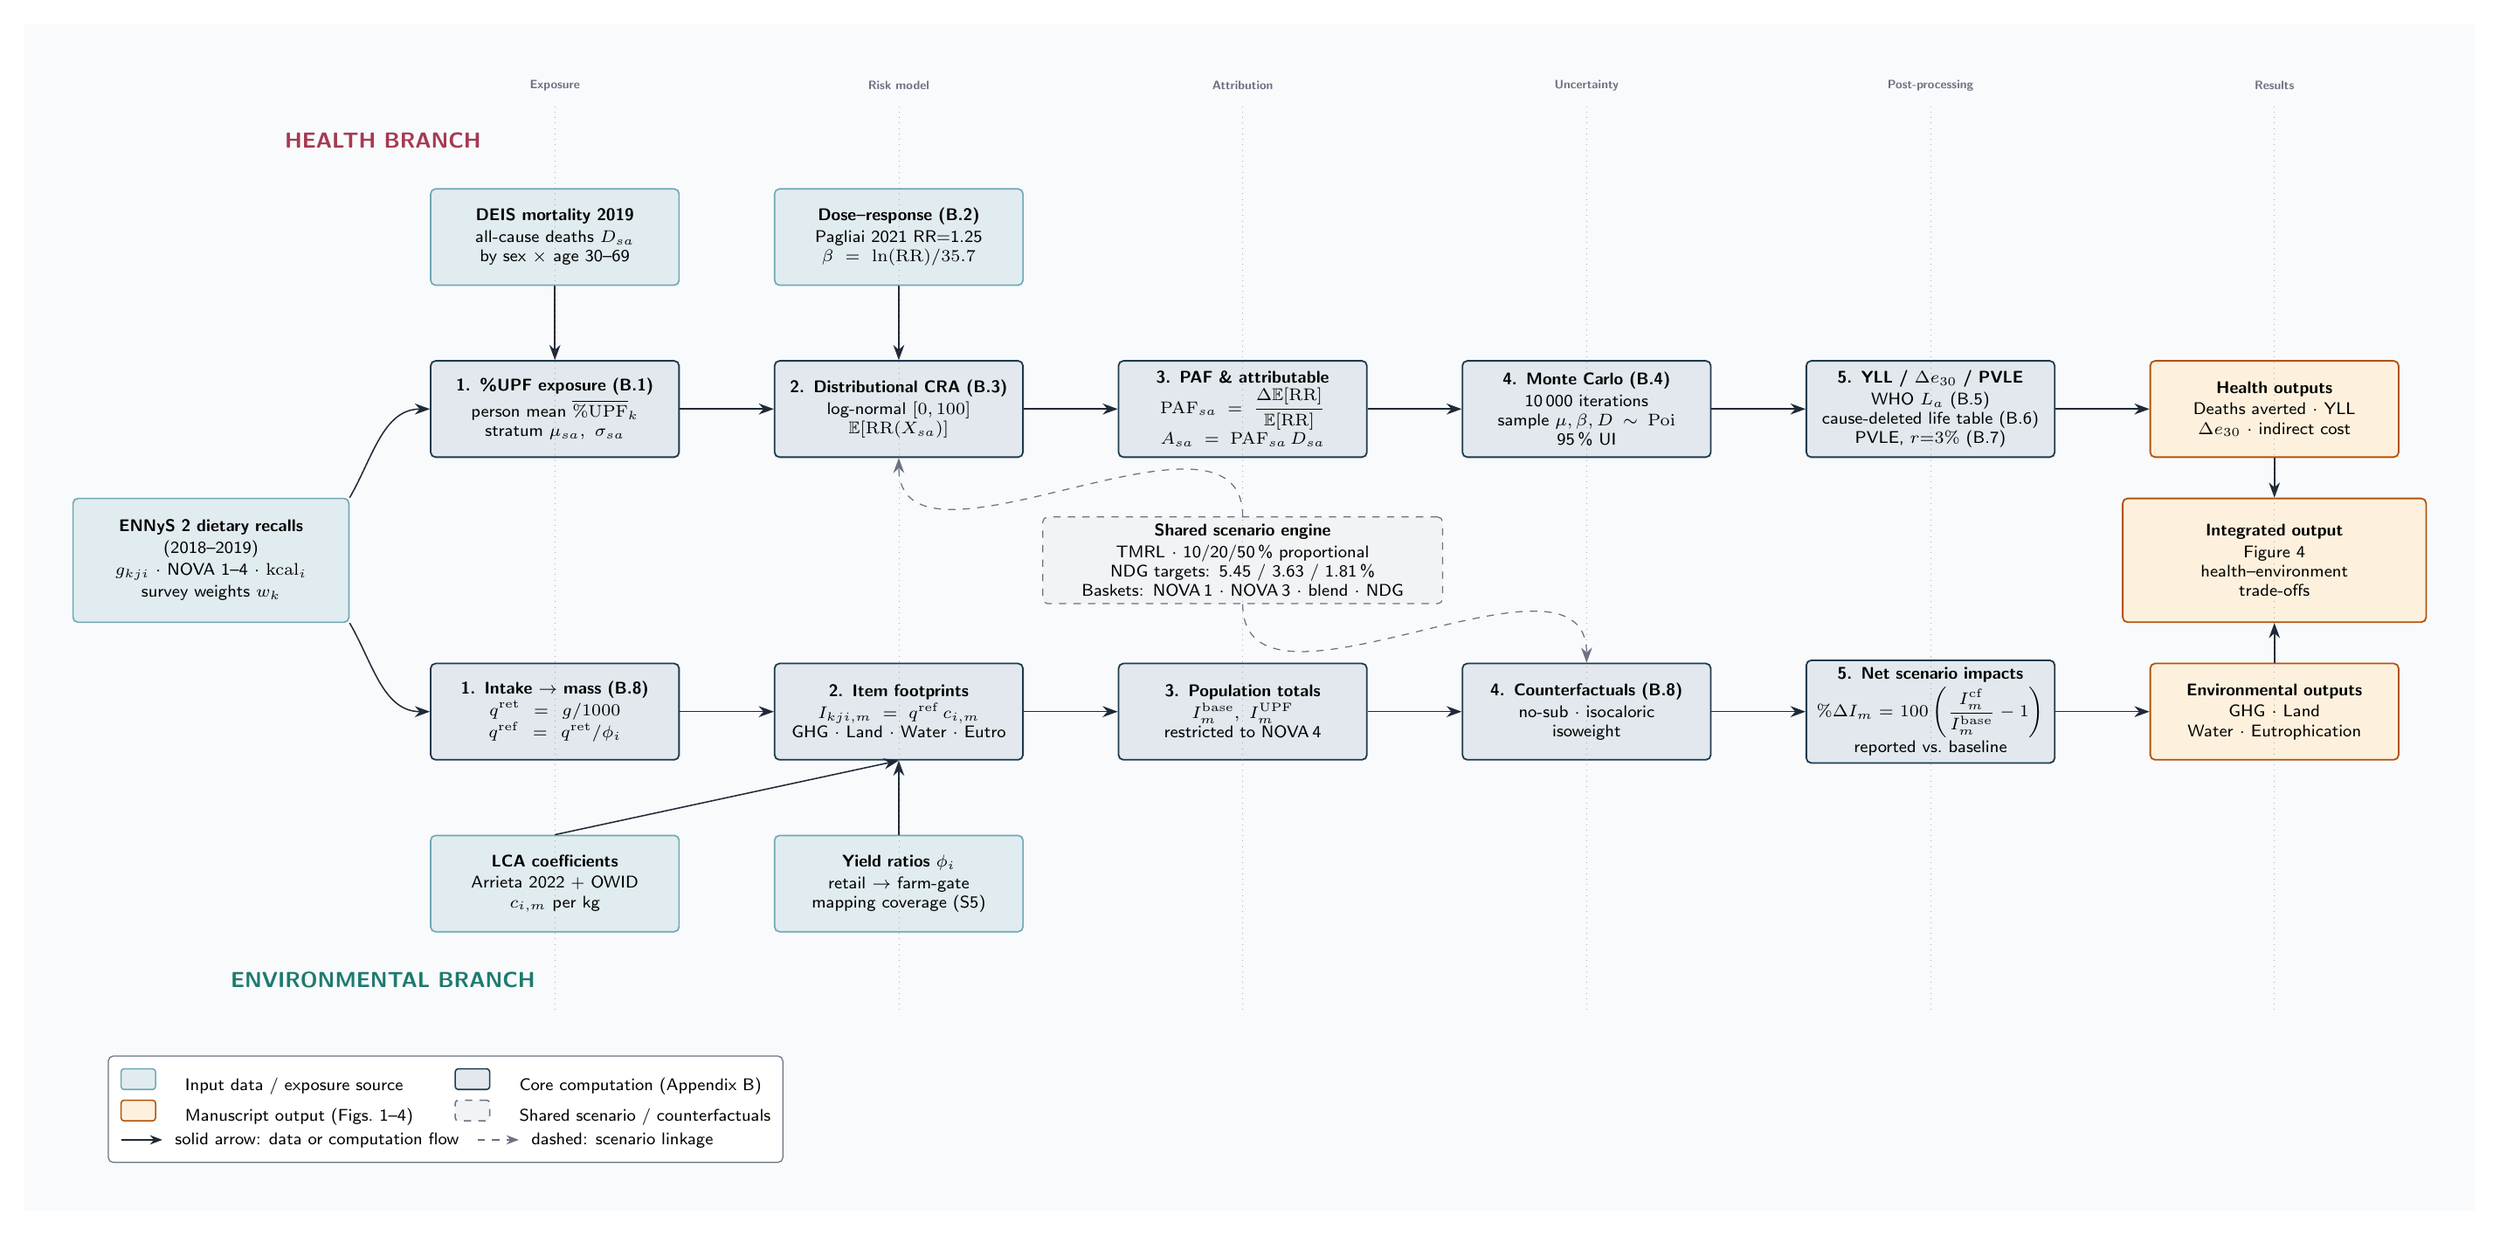
\begin{tikzpicture}[
    x=1cm, y=1cm,
    font=\sffamily\scriptsize,
    >={Stealth[length=2.2mm,width=1.6mm]},
    every node/.style={align=center},
    input/.style  = {draw=cInput,  fill=cInputBg,  line width=0.6pt,
                     rounded corners=2pt, inner sep=3pt,
                     text width=34mm, minimum height=14mm},
    core/.style   = {draw=cCore,   fill=cCoreBg,   line width=0.65pt,
                     rounded corners=2pt, inner sep=3pt,
                     text width=34mm, minimum height=14mm},
    output/.style = {draw=cOutput, fill=cOutputBg, line width=0.65pt,
                     rounded corners=2pt, inner sep=3pt,
                     text width=34mm, minimum height=14mm},
    note/.style   = {draw=cNote, dashed, fill=cNoteBg, line width=0.45pt,
                     rounded corners=2pt, inner sep=3pt,
                     text width=48mm, minimum height=12mm},
    header/.style = {font=\sffamily\bfseries\small},
    flow/.style   = {->, draw=cRule, line width=0.55pt},
    sflow/.style  = {->, draw=cNote, line width=0.45pt, dashed},
    swatch/.style = {rounded corners=1.2pt, line width=0.55pt,
                     minimum width=5mm, minimum height=3mm, inner sep=0pt},
]

% ============================== ROOT =======================================
\node[input, text width=38mm, minimum height=18mm] (root) at (0, 0) {%
  \textbf{ENNyS 2 dietary recalls}\\[1pt]
  (2018--2019)\\[1pt]
  \scriptsize $g_{kji}\ \cdot\ $NOVA 1--4 $\cdot\ \mathrm{kcal}_i$\\[1pt]
  \scriptsize survey weights $w_k$};

% ========================== HEALTH BRANCH (top) ============================
\node[input]  (hAux1) at (5, 4.7)
  {\textbf{DEIS mortality 2019}\\[1pt]
   \scriptsize all-cause deaths $D_{sa}$\\
   \scriptsize by sex $\times$ age 30--69};

\node[input]  (hAux2) at (10, 4.7)
  {\textbf{Dose--response (B.2)}\\[1pt]
   \scriptsize Pagliai 2021 RR=1.25\\
   \scriptsize $\beta=\ln(\mathrm{RR})/35.7$};

\node[core]   (hExp) at (5, 2.2)
  {\textbf{1. \%UPF exposure (B.1)}\\[1pt]
   \scriptsize person mean $\overline{\%\mathrm{UPF}}_k$\\
   \scriptsize stratum $\mu_{sa},\ \sigma_{sa}$};

\node[core]   (hCra) at (10, 2.2)
  {\textbf{2. Distributional CRA (B.3)}\\[1pt]
   \scriptsize log-normal $[0,100]$\\
   \scriptsize $\mathbb{E}[\mathrm{RR}(X_{sa})]$};

\node[core]   (hPaf) at (15, 2.2)
  {\textbf{3. PAF \& attributable}\\[1pt]
   \scriptsize $\mathrm{PAF}_{sa}=\dfrac{\Delta\mathbb{E}[\mathrm{RR}]}{\mathbb{E}[\mathrm{RR}]}$\\
   \scriptsize $A_{sa}=\mathrm{PAF}_{sa}\,D_{sa}$};

\node[core]   (hMc)  at (20, 2.2)
  {\textbf{4. Monte Carlo (B.4)}\\[1pt]
   \scriptsize 10\,000 iterations\\
   \scriptsize sample $\mu,\beta,D\sim\mathrm{Poi}$\\
   \scriptsize 95\,\% UI};

\node[core]   (hPost) at (25, 2.2)
  {\textbf{5. YLL / $\Delta e_{30}$ / PVLE}\\[1pt]
   \scriptsize WHO $L_a$ (B.5)\\
   \scriptsize cause-deleted life table (B.6)\\
   \scriptsize PVLE, $r{=}3\%$ (B.7)};

\node[output] (hOut) at (30, 2.2)
  {\textbf{Health outputs}\\[1pt]
   \scriptsize Deaths averted $\cdot$ YLL\\
   \scriptsize $\Delta e_{30}$ $\cdot$ indirect cost};

% ======================== ENVIRONMENTAL BRANCH (bottom) ====================
\node[input]  (eAux1) at (5, -4.7)
  {\textbf{LCA coefficients}\\[1pt]
   \scriptsize Arrieta 2022 + OWID\\
   \scriptsize $c_{i,m}$ per kg};

\node[input]  (eAux2) at (10, -4.7)
  {\textbf{Yield ratios $\phi_i$}\\[1pt]
   \scriptsize retail $\to$ farm-gate\\
   \scriptsize mapping coverage (S5)};

\node[core]   (eMass) at (5, -2.2)
  {\textbf{1. Intake $\to$ mass (B.8)}\\[1pt]
   \scriptsize $q^{\mathrm{ret}}=g/1000$\\
   \scriptsize $q^{\mathrm{ref}}=q^{\mathrm{ret}}/\phi_i$};

\node[core]   (eItem) at (10, -2.2)
  {\textbf{2. Item footprints}\\[1pt]
   \scriptsize $I_{kji,m}=q^{\mathrm{ref}}\,c_{i,m}$\\
   \scriptsize GHG $\cdot$ Land $\cdot$ Water $\cdot$ Eutro};

\node[core]   (eAgg)  at (15, -2.2)
  {\textbf{3. Population totals}\\[1pt]
   \scriptsize $I^{\mathrm{base}}_m,\ I^{\mathrm{UPF}}_m$\\
   \scriptsize restricted to NOVA\,4};

\node[core]   (eCf)   at (20, -2.2)
  {\textbf{4. Counterfactuals (B.8)}\\[1pt]
   \scriptsize no-sub $\cdot$ isocaloric\\
   \scriptsize isoweight};

\node[core]   (ePost) at (25, -2.2)
  {\textbf{5. Net scenario impacts}\\[1pt]
   \scriptsize $\%\Delta I_{m}=100\left(\dfrac{I^{\mathrm{cf}}_{m}}{I^{\mathrm{base}}_{m}}-1\right)$\\
   \scriptsize reported vs.\ baseline};

\node[output] (eOut)  at (30, -2.2)
  {\textbf{Environmental outputs}\\[1pt]
   \scriptsize GHG $\cdot$ Land\\
   \scriptsize Water $\cdot$ Eutrophication};

% ========================= SCENARIO ENGINE (centre) ========================
\node[note, text width=56mm] (scen) at (15, 0)
  {\textbf{Shared scenario engine}\\[1pt]
   \scriptsize TMRL $\cdot$ 10/20/50\,\% proportional\\
   \scriptsize NDG targets: 5.45 / 3.63 / 1.81\,\%\\
   \scriptsize Baskets: NOVA\,1 $\cdot$ NOVA\,3 $\cdot$ blend $\cdot$ NDG};

% ===================== FINAL INTEGRATED OUTPUT =============================
\node[output, text width=42mm, minimum height=18mm] (final) at (30, 0)
  {\textbf{Integrated output}\\[1pt]
   \scriptsize Figure 4\\
   \scriptsize health--environment\\
   \scriptsize trade-offs};

% ================================ EDGES ===================================
% Root -> first stage of each branch
\draw[flow] (root.north east) to[out=60,  in=180] (hExp.west);
\draw[flow] (root.south east) to[out=-60, in=180] (eMass.west);

% Auxiliary inputs feeding their relevant step
\draw[flow] (hAux1.south) -- (hPaf.north -| hAux1.south);
\draw[flow] (hAux2.south) -- (hCra.north);
\draw[flow] (eAux1.north) -- (eItem.south);
\draw[flow] (eAux2.north) -- (eAgg.south -| eAux2.north);

% Health branch horizontal flow
\draw[flow] (hExp.east)  -- (hCra.west);
\draw[flow] (hCra.east)  -- (hPaf.west);
\draw[flow] (hPaf.east)  -- (hMc.west);
\draw[flow] (hMc.east)   -- (hPost.west);
\draw[flow] (hPost.east) -- (hOut.west);

% Env branch horizontal flow
\draw[flow] (eMass.east) -- (eItem.west);
\draw[flow] (eItem.east) -- (eAgg.west);
\draw[flow] (eAgg.east)  -- (eCf.west);
\draw[flow] (eCf.east)   -- (ePost.west);
\draw[flow] (ePost.east) -- (eOut.west);

% Scenario engine feeds the CRA node (health) and counterfactuals (env)
\draw[sflow] (scen.north) to[out=90,  in=-90] (hCra.south);
\draw[sflow] (scen.south) to[out=-90, in=90]  (eCf.north);

% Convergence of branch outputs onto the integrated output
\draw[flow] (hOut.south) to[out=-90, in=90]  (final.north);
\draw[flow] (eOut.north) to[out=90,  in=-90] (final.south);

% ============================ BRANCH HEADERS ================================
\node[header, text=cHealth] at (2.5, 6.1) {HEALTH BRANCH};
\node[header, text=cEnv]    at (2.5, -6.1) {ENVIRONMENTAL BRANCH};

% Subtle horizontal rails behind branch rows
\begin{pgfonlayer}{background}
  \draw[cHealth, line width=0.45pt, dashed, opacity=0.40]
    (3.0,  2.2) -- (32.0,  2.2);
  \draw[cEnv,    line width=0.45pt, dashed, opacity=0.40]
    (3.0, -2.2) -- (32.0, -2.2);
\end{pgfonlayer}

% ============================ STAGE HEADERS (top) ==========================
\foreach \x/\lbl in {5/Exposure,10/Risk model,15/Attribution,20/Uncertainty,25/Post-processing,30/Results}{
  \node[font=\sffamily\bfseries\tiny, text=cNote] at (\x, 6.9) {\lbl};
  \draw[cNote, line width=0.25pt, dotted, opacity=0.55]
    (\x, 6.6) -- (\x, -6.6);
}

% ============================== LEGEND =====================================
% Legend uses actual node styling (bg fill + colored border) so that the
% swatches match what the reader sees in the diagram, not just accent colors.
\node[draw=cNote, line width=0.45pt, rounded corners=2pt,
      inner sep=5pt, fill=white, font=\sffamily\scriptsize,
      anchor=north west] (legend) at (-1.5, -7.2) {%
  \begin{tabular}{@{}c l @{\hspace{6mm}} c l@{}}
    \tikz\node[swatch,draw=cInput, fill=cInputBg]{};   & Input data /
      exposure source &
    \tikz\node[swatch,draw=cCore, fill=cCoreBg]{};     & Core computation
      (Appendix B) \\[1.5pt]
    \tikz\node[swatch,draw=cOutput,fill=cOutputBg]{};  & Manuscript output
      (Figs.\ 1--4) &
    \tikz\node[swatch,draw=cNote, fill=cNoteBg, dashed]{}; & Shared scenario
      / counterfactuals \\[1.5pt]
    \multicolumn{4}{@{}l}{%
       \tikz\draw[->, draw=cRule, line width=0.55pt, >={Stealth[length=1.8mm]}]
            (0,0) -- (6mm,0);\ \ solid arrow: data or computation flow\quad
       \tikz\draw[->, draw=cNote, line width=0.45pt, dashed,
                  >={Stealth[length=1.8mm]}]
            (0,0) -- (6mm,0);\ \ dashed: scenario linkage}
  \end{tabular}};

% ============================ BACKGROUND ===================================
\begin{pgfonlayer}{background}
  \node[fill=cBg, inner sep=7mm,
        fit=(root)(hAux1)(hOut)(eAux1)(eOut)(final)(legend)
            (current bounding box)] {};
\end{pgfonlayer}

\end{tikzpicture}
\end{document}
